%\chapter{\acl{mipwa}}
\chapter{\texorpdfstring{\Acl{mipwa}}{Model-independent PWA}}
\label{chap:model_independent_pwa}

By means of a \acf{mipwa} one can study decays whose wave resonance content is not yet well known or whose resonance shapes are not yet precisely understood.
\citeauthor{PhysRevD.73.032004}, at Fermilab, first performed a \ac{mipwa} of a heavy-meson decay to parametrize the S-wave component of the $\PKminus{}\Ppiplus{}$ system in the $\PDplus\to\PKminus\Ppiplus\Ppiplus$ decay~\cite{PhysRevD.73.032004}.
\citeauthor{Link200914}, in the \focus{} collaboration, conducted a similar study on the same hadronic decay~\cite{Link200914}.


In this chapter, I will describe a utility I coded, which implements the \ac{mipwa} formalism.\marginpar{\centering\qrcode[height=2cm]{https://github.com/pdigiglio/ModelIndependentFit}\captionof*{figure}{Fit utility's \textsc{url}.}}
The utility is based on \pac{yap}---for the calculation of the decay amplitudes---and \pac{bat}---for the sampling of the phase space.
I will also show the result of the fits I performed on \ac{mc} data of $\PDplus\to\Ppiplus\Ppiminus\Ppiplus$ decays to test the utility.
The project is hosted on \textsf{GitHub} at \url{https://github.com/pdigiglio/ModelIndependentFit}.


    \section{The fit utility}

    The \ac{mipwa} utility implements a \pac{yap} decay model in which the dynamic shape of each isobar is a piecewise function.\footnote{So far, I did not yet implement the mixed formalism with freed and fixed waves.}
    The model assigns a non-fixed free amplitude to each mass bin of the dynamic shapes.
    The non-fixed free amplitudes are then mapped to fit parameters for the \pac{bat} sampler.
    \pac{bat} queries the model likelihood, and updates the fit parameters---and, consequently, the non-fixed free amplitudes of the \pac{yap} model---until it finds a maximum of the likelihood.


    Please note that unlike chapter~\ref{chap:yap}, where I reserved the word ``parameter'' to indicate the smart variables the \lstinline!MassShape! class depends on, here I will also call ``parameter'' a fit \ac{dof}.

    \subsection{The decay model}

    As of now, \pac{yap} does not yet provide the piecewise dynamic shape in equation~\eqref{eq:step_dynamic_shape}, which is needed to perform a \ac{mipwa} of a decay.
    However, such a dynamic shape can be constructed in \pac{yap} starting from the formal analogy between the model-independent decay amplitude in equation~\eqref{eq:freed_wave_amplitude}---the one that has to be fit to the data---and the model-dependent decay amplitude in equation~\eqref{eq:non_redundant_model_dependent_isobar_decomposition}.
    In fact, equation~\eqref{eq:freed_wave_amplitude} also applies to a decay proceeding through $N_\text{bins}$ intermediate states, $\xi_i$, whose dynamic shape is a characteristic function, such that
    \begin{equation}
        \PDplus\to\xi_i\Ppiplus,\quad%\text{ and }
        \xi_i\to\Ppiminus\Ppiplus,\quad
        \text{with } i \in \set{1,\dots, N_{\text{bins}}}.
    \end{equation}
    Therefore, in the model to fit to the data, each wave contains as many artificial resonances as the bins of the mass range.
    The dynamic shape of each resonance is the \lstinline!MassBin! class presented in listing~\ref{lst:mass_shape}, page~\pageref{lst:mass_shape}.
    This means that every bin in figure~\ref{fig:step_function_approximation}, where I show a binning example of a Breit-Wigner distribution, corresponds to a different decay mode of the parent particle.
    After the model is locked, each resonance will be assigned a non-fixed free amplitude to be handed over to \pac{bat} for the fit stage.


    Please note that the \lstinline!free_amplitudes! function in \pac{yap} returns an unsorted \lstinline!std::set! of pointers to the free amplitudes of the decay model.\footnote{The \lstinline!std::set! is a sorted container but---in this case---its elements are sorted by their memory address.}
    Thus, the fit utility makes sure that they do not get internally displaced at runtime and can always be associated to the correct bin.
    While the mass bins can be sorted by checking their boundaries, there is no natural way to sort the free amplitudes.
    So I stored them in a \lstinline!std::vector! and sorted them by their index in the vector.
    \begin{figure}
        \centering
        \subfloat[][]{\begin{tikzpicture}
    \begin{axis}[
        amplitude_plot,
        width = .7\textwidth,
        xlabel={$m_{\pi^+\pi^-}$ [\si{\giga\electronvolt^2\per\c^4}]},
    ]
        \pgfmathsetmacro{\m}{.98}
        \pgfmathsetmacro{\T}{.07}
        \addplot+ [guess, domain={.279:1.73}, samples=100, smooth] gnuplot {1./sqrt((\m * \m - x * x)**2 + (\m * \T)**2)};
        
        \addplot+ [fit, mark=none] table {data/dalitz_displaced/binned_breit-wigner_displaced.txt};
    \end{axis}
\end{tikzpicture}
}

        \subfloat[][]{\begin{tikzpicture}
    \begin{axis} [dalitz_plot]

        \addplot3 [dalitz]
          gnuplot [raw gnuplot] { splot "data/dalitz_displaced/f0_displaced_mcmc.txt" using 1:2:3 };
    \end{axis}
\end{tikzpicture}
}

        \caption{Effect of the displacement of the fourth and the fourteenth free amplitudes.}
        \label{fig:bw_binning_displaced}
    \end{figure}
    Figure~\ref{fig:bw_binning_displaced} shows the effect of the displacement of two free amplitudes.


    %Then I create a \lstinline!Model! for a decay of a $\PDplus$ to $\xi_i\Ppiminus$, with the $\xi_i$ decaying itself to $\Ppiplus\Ppiminus$ and having a \lstinline!MassBin! dynamic shape: $\Characteristic_{B_i}$.
    %I make sure that $\set{B_i}$ is a partition of the allowed mass range of the $\Ppiplus\Ppiminus$, namely that
    %\begin{equation}
    %    \bigcup_{i=0}^{N_\text{bins}-1} B_i = [2m_{\pi},m_{\PD}-m_{\pi})
    %\end{equation}
    %Locking the model will associate a free amplitude to each dynamic shape.

    
    %It is very important for the fit to work correctly that the free amplitudes do not get internally displaced and can always be associated to the correct mass bin.
    %While the mass bins can be sorted by checking at their boundaries, there is no natural way to sort the free amplitudes.
    %So I placed them in a \lstinline!std::vector! and sorted them by their index in the vector.
    %\begin{figure}
    %    \centering
    %    \subfloat[][]{\begin{tikzpicture}
    \begin{axis}[
        amplitude_plot,
        width = .7\textwidth,
        xlabel={$m_{\pi^+\pi^-}$ [\si{\giga\electronvolt^2\per\c^4}]},
    ]
        \pgfmathsetmacro{\m}{.98}
        \pgfmathsetmacro{\T}{.07}
        \addplot+ [guess, domain={.279:1.73}, samples=100, smooth] gnuplot {1./sqrt((\m * \m - x * x)**2 + (\m * \T)**2)};
        
        \addplot+ [fit, mark=none] table {data/dalitz_displaced/binned_breit-wigner_displaced.txt};
    \end{axis}
\end{tikzpicture}
}

    %    \subfloat[][]{\begin{tikzpicture}
    \begin{axis} [dalitz_plot]

        \addplot3 [dalitz]
          gnuplot [raw gnuplot] { splot "data/dalitz_displaced/f0_displaced_mcmc.txt" using 1:2:3 };
    \end{axis}
\end{tikzpicture}
}

    %    \caption{Effect of the displacement of the fourth and the fourteenth free amplitudes.}
    %    \label{fig:bw_binning_displaced}
    %\end{figure}
    %Figure~\ref{fig:bw_binning_displaced} shows the effect of the displacement of two free amplitudes.
    %This can happen because the \lstinline!free_amplitudes! function in \pac{yap} returns an unsorted \lstinline!std::set! of pointers to the free amplitudes of the decay model.\footnote{The \lstinline!std::set! is a sorted container but---in this case---its elements are sorted by their memory address.}


    %For this reason, I implemented the \lstinline!MassBin! dynamic shape shown in listing~\ref{lst:mass_shape}.

    \subsection{The fit \acp{dof}}

    To perform the fit, I have developed a back-end to \lstinline!BCModel!, the \pac{bat} class that sets the fit parameters up and reports the logarithm of the likelihood.


    As \pac{bat} can only handle real fit \acp{dof}, I introduce an invertible map between the complex free amplitudes---the $\gamma_{(I,i)}$ coefficients of the decay model in equation~\eqref{eq:freed_wave_amplitude}---and the fit parameters, $\Phi\colon \C\to\R\x\R$.


    The quantity that describes the input data to fit the model to is the decay intensity,
    \begin{equation}\label{eq:intensity_phase_ambiguity}
        \Intensity(\tau) = \abs{\A(\tau)}^2 = \abs{\eu^{\iu\phi}\A(\tau)}^2,
        \quad
        \text{with }
        \phi\in\R.
    \end{equation}
    Because of the continuous ambiguity in the right-hand equality of equation~\eqref{eq:intensity_phase_ambiguity}, the representation of a complex number by its magnitude and phase,
    \begin{equation}
        \Phi(\gamma) \coloneqq (\abs{\gamma}, \arg\gamma),
    \end{equation}
    is not suited for the fit parameters.
    In fact, if the vector $(\tilde \gamma_0, \dots, \tilde \gamma_{N_\text{bins}-1})$ of free amplitudes maximises the model likelihood, any rotation of its elements in the complex plane, $(\exp(\iu\phi)\,\tilde \gamma_0, \dots, \exp(\iu\phi)\,\tilde \gamma_{N_\text{bins}-1})$, does.
    Moreover, \pac{bat} cannot properly sample the phase space of a periodic variable.\marginpar{\color{red} why?}
    The ambiguity in equation~\eqref{eq:intensity_phase_ambiguity} can be avoided by fixing one of the bin phases to a fixed value, \eg~$\arg \gamma_0 \equiv 0$.


    Another ambiguity is
    \begin{equation}\label{eq:intensity_conjugate_ambiguity}
        \abs{\A(\tau)}^2 = \abs{\A^*(\tau)}^2.
    \end{equation}
    As all the terms in the decay amplitude in equation~\eqref{eq:freed_wave_amplitude} are real, to the vector $(\tilde \gamma_0, \dots, \tilde \gamma_{N_\text{bins}-1})$ corresponds $(\tilde \gamma_0^*, \dots, \tilde \gamma_{N_\text{bins}-1}^*)$
    \begin{equation}
        \Phi(\gamma) = (\Re(\gamma), \Im(\gamma))
    \end{equation}

    When choosing the representation of the complex fit parameters


    To choose the fit-parameter representation, I note that both the decay amplitude in equation~\eqref{eq:isobar_decomposition} and its complex conjugate squared give the same event intensity:
    \begin{equation}
        \abs{\A(\tau)}^2 = \abs{\A^*(\tau)}^2.
    \end{equation}

    The representation of a complex number in terms of its real and imaginary parts, $\Phi(\gamma) = (\Re(\gamma), \Im(\gamma))$, is not suited.
    In the particular case of the decay amplitude in the \ac{mipwa} formalism, all the functions in the amplitude are real, so there is an ambiguity.





    The first test fit I performed is to the data of the $\PDplus\to(\Pfnez\to\Ppiplus\Ppiminus)\Ppiplus$ decay, shown in Dalitz plot~\ref{fig:dalitz_f0_980_only_source}.
    \begin{figure}
        \centering
        \begin{tikzpicture}
    \begin{axis}[
            xlabel = {$\Re (\Delta_{\Pfnez}^{\text{BW}}(s))$ [\si{1/(\giga\electronvolt/\c^2)^2}]},
            ylabel = {$\Im (\Delta_{\Pfnez}^{\text{BW}}(s))$ [\si{1/(\giga\electronvolt/\c^2)^2}]},
        ]

        \pgfmathsetmacro{\m}{.98}
        \pgfmathsetmacro{\T}{.07}

        \addplot+ [black, mark options={mark size = .75, color=black}]
          gnuplot [raw gnuplot] {
            set parametric;
            f(x) = 1. / (\m * \m - x * x - {0., 1.} * \m * \T);
            set samples 150;
            plot [.279:1.73] real(f(t)), imag(f(t));
        };
    \end{axis}
\end{tikzpicture}

        \caption{Argand-Gau\ss{} plot of a non-relativistic Breit-Wigner~\eqref{eq:bw}.}
        \label{fig:bw_argand_gauss}
    \end{figure}
    The decay proceeds through the \Pfnez{} resonance only with non-relativistic Breit-Wigner dynamic shape, whose plot in the Argand-Gau\ss{} plane is shown in figure~\ref{fig:bw_argand_gauss}.
    \begin{equation}
        \Phi(\gamma) = (\abs{\gamma}, \arg\gamma)
    \end{equation}
    I can exploit the fact that the fit parameters have a fixed position in the vector:
    \begin{equation}
        \Phi(\gamma_0) = (\abs{\gamma_0}, 0)
    \end{equation}
    \begin{equation}
        \Phi(\gamma_0,\dots,\gamma_j) = (\abs{\gamma_j}, \arg(\gamma_j) - \arg(\gamma_{j-1})), \text{ so that }\phi_j = \sum_{i=0}^j \uD \phi_i
    \end{equation}



    I am fitting the amplitude~\eqref{eq:freed_wave_amplitude} to the data.


    In the $\Phi(\gamma) = (\abs{\gamma}, \arg\gamma)$ representation, there is the phase ambiguity and the conjugate ambiguity.


    The first fit I performed is the decay of the $\Pfnez$.
    The real-imaginary representation of the free amplitudes proved inconvenient as the data is ambiguous.

    In the first fit attempt, I represented the free amplitudes by their real and imaginary parts.
    With this choice, the pre-run did not converge as there is an ambiguity in the sign of the imaginary part of the parameters.
    In fatc, for each set of parameters $\Set{(\Re,\Im)_i}$ that maximizes the likelihood, also $\Set{(\Re,-\Im)_i}$ does.


    As the plot~\ref{fig:bw_argand_gauss} shows, the angle is increasing.






    \subsection{Likelihood function}

    The model-independent fit to the \ac{mc}-generated data set, $D = \Set{d_1, d_2,\dots, d_m}$, is performed through the maximum-likelihood method.
    In this section I am going to justify the expression of the log-likelihood used in the fittin routine.

    If $p \coloneqq (p_1, p_2,\dots, p_n)$ is the fit-parameter vector, the Bayes' theorem reads
    \begin{equation}
        P(p\given D) = \frac{P(D\given p)\, P(p)}{P(D)}.
    \end{equation}
    First, let's note that the parameters are assumed to be independent among each other, so that
    \begin{equation}
        P(p) = \prod_{i = 1}^n P_i(p_i),
    \end{equation}
    being $P_i$ the probability density function of the $i$-th parameter.
    As there is no information about the fit parameters, I choose the following flat distributions for the priors:
    \begin{equation}\label{eq:flat_priors}
        P_i(p_i) =
        \begin{cases}
            1/(b_i - a_i) & \text{if } a_i \le p_i \le b_i, \\
            0             & \text{otherwise},
        \end{cases}
    \end{equation}
    where $[a_i, b_i]$ is the domain of the $i$-th parameter.
    This choice implies that the prior $P(p)$ is a constant function in the hypercube where all its arguments are defined.

    The likelihood function is defined as the conditional probability of observing the data set $D$ given $p$, that is
    \begin{equation}
        L(p) \coloneqq P(D\given p).
    \end{equation}
    Since the priors and $P(D)$ are constant functions, the likelihood is directly proportional to the posterior probability:
    \begin{equation}
        P(p\given D) = \alpha L(p),\quad \text{where } \alpha \coloneqq \frac{P(p)}{P(D)}.
    \end{equation}
    The logarithm of the likelihood reads
    \begin{equation}
        \log L(p) = \log P(p\given D) - \log \alpha.
    \end{equation}


    The posterior probability is proportional to the square magnitude of the decay amplitude, which is the model \emph{intensity}\index{intensity}.
    This is a function of the decay phase-space point $\mu$ defined as follows:
    \begin{equation}
        I_p(\mu) \coloneqq \abs{\A_p(\mu)}^2.
    \end{equation}
    With this definition, the posterior probability of the fit parameters given an observed point in the phase space, $d$, is
    \begin{equation}
        P(p\given d) = \frac{I_p(d)}{\displaystyle\int I_p(\mu)\ud\mu},
    \end{equation}
    where the normalizing integral is over the whole decay phase-space.
    Assuming the point in the observed data set have no correlation, the posterior for the fit parameters given the whole set $D$ is
    \begin{equation}
        P(p\given D) = \prod_{d\in D} P(p\given d) = \frac{\displaystyle\prod_{d\in D}I_p(d)}{\displaystyle\left(\int I_p(\mu)\ud\mu\right)^m}.
    \end{equation}
    The log-likelihood then reads
    \begin{equation}
        \log L(p) = \sum_{d\in D}\log I_p(d) - m\log\int I_p(\mu) \ud \mu - \log \alpha.
    \end{equation}
    Retaining only the $p$-dependent terms in the equation above, the expression of the log-likelihood that needs to be maximized is
    \begin{equation}\label{eq:log_lik_unstable}
        \log \tilde L(p) = \sum_{d\in D}\log I_p(d) - m\log \int I_p(\mu)\ud\mu.
    \end{equation}


    It is worth pointing out that, in the fit routine, the expression used for the log-likelihood is the following:
    \begin{equation}\label{eq:log_lik_stable}
        \log \tilde L(p) = \sum_{d\in D}\left(\log I_p(d) - \log \int I_p(\mu)\ud\mu\right)\!.
    \end{equation}
    In fact, while being mathematically equivalent, the~\eqref{eq:log_lik_stable} is numerically more stable than the~\eqref{eq:log_lik_unstable}.


    \subsection{The user interface}
    \begin{figure}
        \centering
        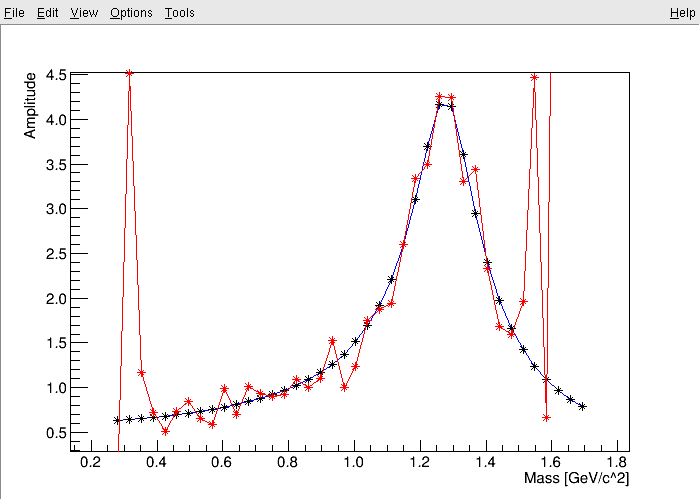
\includegraphics[width=.9\textwidth]{fig/f2_real_time_fit.png}

        \caption[Screenshot of the real-time plot of a decay-amplitude magnitude.]{Screenshot of the real-time plot of the decay-amplitude magnitude while fitting a \Pfii{} resonance.
                 In blue, with black points, the initial guess for the fit parameters; in red, the current values of the fit parameters.}
                 %In this case, the initial guess for the fit parameters is the value of the \Pfii{} dynamic shape on the low edges of the bins that partition the mass range.}
        \label{fig:rt_par_fit}
    \end{figure}


    Due to the long fit runtimes, I implemented a real-time visualization tool with \ROOT{}.
    For each freed wave, the fit utility will create two canvases: one plots the dynamic-shape magnitude, the other the dynamc-shape phase.
    Each canvas contains two \ROOT{} graphs: the initial guess for the fit parameters, and the values of the fit parameters.
    The latter graph gets updated in real time at every fit iteration.
    Figure~\ref{fig:rt_par_fit} shows a screenshot of the dynamic-shape magnitude of a D wave (containing, in this case, a \Pfii{} resonance only).
    Looking at these canvas, the user can realize if there is some mistake in the fit without having to wait until it ends.

    \section{Fits}

    In this section I present the fits I performed by means of the utility described above.
    I generated the data to fit the model to using \pac{bat} as a \ac{mc} engine, and \pac{yap} as an amplitude calculator.
    Listing~\ref{lst:partial_cleo_decay} shows how to set up a \lstinline!Model! instance whose decay intensity can be used as the \ac{mc} sampling distribution to generate the data.


    In the following plots, first, I show the fits of phase motion (\eg~figure~\ref{fig:f0_only_phase_fit}) and dynamic-shape magnitude (\eg~figure~\ref{fig:f0_only_magnitude});
    then, a comparison between the source \ac{mc} data (\eg~figure~\ref{fig:dalitz_f0_980_only_source}) and a set of \ac{mc} data generated according to the model-independent decay amplitude whose parameters are fixed to the ones extracted from the fit (\eg~figure~\ref{fig:dalitz_f0_980_only_result}).
    Please note that in figure~\ref{fig:f0_only}, as in all the following fit plots, the bin error bars are on the left edge of the bin they refer to.


    \subsection{Single-resonance Dalitz plots}

    % -- f0(980) ----------------------------------------------------------
    \begin{figure}
        \centering
        \subfloat[][\label{fig:f0_only_phase_fit}]{\begin{tikzpicture}
    \begin{axis}[phase_plot]
        \addplot+ [guess] table [x index={0}, y index={5}] {data/f2/par_guess.txt};
        \addplot+ [fit] table [x index={0}, y index={5}, y error index={6}]
                  {data/f2/par_fit.txt};

    \end{axis}
\end{tikzpicture}
}

        \subfloat[][\label{fig:f0_only_magnitude}]{\begin{tikzpicture}
    \begin{axis}[amplitude_plot]
        \addplot+ [guess] table [x index={0}, y index={1}] {data/f0/par_guess.txt};
        \addplot+ [fit] table [x index={0}, y index={1}, y error index={2}]
                  {data/f0/par_fit.txt};
    \end{axis}
\end{tikzpicture}

}
        \caption{Freed-wave fit of the S wave of a $\PDplus \to \Ppiplus\Ppiminus\Ppiplus$ decay through the \Pfnez{} resonance.~\Square} 
        \label{fig:f0_only}
    \end{figure}
    \begin{figure}
        \centering
        \subfloat[][Source data: decay in the S wave through the \Pfnez{} resonance.\label{fig:dalitz_f0_980_only_source}]{\begin{tikzpicture}
    \begin{axis} [dalitz_plot]

        \addplot3 [dalitz]
          gnuplot [raw gnuplot] { splot "data/f2/f2_mcmc.txt" using 1:2:3 };
    \end{axis}
\end{tikzpicture}
}

        \subfloat[][Result of the model-independent fit to the plot shown above.\label{fig:dalitz_f0_980_only_result}]{\begin{tikzpicture}
    \begin{axis} [dalitz_plot]
        \addplot3 [dalitz]
          gnuplot [raw gnuplot]
                  { splot "data/f0_f0_1500_sigma_rho0/f0_f0_1500_sigma_rho0_fit_result_mcmc.txt" using 1:2:3 };
    \end{axis}
\end{tikzpicture}
}
        \caption{\ac{mc}-generated Dalitz plots of a $\PDplus \to \Ppiplus\Ppiminus\Ppiplus$ decay.~\Square}
        \label{fig:f0_only_dalitz}
    \end{figure}
    % ---------------------------------------------------------------------
    In this section, I present the test fits I performed on data sets where the $\PDplus\to\Ppiplus\Ppiminus\Ppiplus$ decay proceeds through one intermediate state only. 
    In this case, the dynamic-shape phase is an increasing function of the resonance mass and ranges from $0$ to $\pi$, so I restricted the phase-motion parameter to the asymmetric range $[0,\pi]$.


    First, I show the fits of phase motion (\eg~figure~\ref{fig:f0_only_phase_fit}) and dynamic-shape magnitude (\eg~figure~\ref{fig:f0_only_magnitude});
    then, a comparison between the source \ac{mc} data (\eg~figure~\ref{fig:dalitz_f0_980_only_source}) and a set of \ac{mc} data generated according to the model-independent decay amplitude whose parameters are fixed to the ones extracted from the fit (\eg~figure~\ref{fig:dalitz_f0_980_only_result}).
    Please note that in figure~\ref{fig:f0_only}, as in all the following fit plots, the bin error bars are on the left edge of the bin they refer to.


    Figure~\ref{fig:f0_only} shows the fit performed on the decay proceeding through the $\Pfnez{}$ resonance in the S wave.
    I optimized the mass binning in the neighborhood of the resonance peak.
    This is the easiest possible fit as in the S wave both the spin-dependent part of the decay amplitude and the Blatt-Weisskopf factor are constant over the phase space.
    Figure~\ref{fig:f0_only_dalitz} shows the comparison between the Dalitz plots of the source data and the data generated with the fitted parameters.


    \begin{figure}
        \centering

        \subfloat[][]{\begin{tikzpicture}
    \begin{axis}[phase_plot]
        \addplot+ [guess] table [x index={0}, y index={5}] {data/f2/par_guess.txt};
        \addplot+ [fit] table [x index={0}, y index={5}, y error index={6}]
                  {data/f2/par_fit.txt};

    \end{axis}
\end{tikzpicture}
}

        \subfloat[][]{\begin{tikzpicture}
    \begin{axis}[amplitude_plot]
        \addplot+ [guess] table [x index={0}, y index={1}] {data/f0/par_guess.txt};
        \addplot+ [fit] table [x index={0}, y index={1}, y error index={2}]
                  {data/f0/par_fit.txt};
    \end{axis}
\end{tikzpicture}

}

        \caption{Freed-wave fit of the P wave of a $\PDplus \to \Ppiplus\Ppiminus\Ppiplus$ decay through the \Prhozero{} resonance.~\Star}
        \label{fig:rho0_only}
    \end{figure}
    \begin{figure}
        \centering
        \subfloat[\acs{mc}-generated Dalitz plot of a P-wave decay through the \Prhozero{} resonance.]%
                 [Source data: P-wave decay through the \Prhozero{} resonance.\label{fig:rho0_only_dalitz_source}]%
                 {\begin{tikzpicture}
    \begin{axis} [dalitz_plot]

        \addplot3 [dalitz]
          gnuplot [raw gnuplot] { splot "data/f2/f2_mcmc.txt" using 1:2:3 };
    \end{axis}
\end{tikzpicture}
}

        \subfloat[\acs{mc}-generated Dalitz plot of a P-wave decay through the \Prhozero{} resonance.]%
                 [Result of the model-independent fit to the plot shown above.\label{fig:rho0_only_dalitz_fitted}]%
                 {\begin{tikzpicture}
    \begin{axis} [dalitz_plot]
        \addplot3 [dalitz]
          gnuplot [raw gnuplot]
                  { splot "data/f0_f0_1500_sigma_rho0/f0_f0_1500_sigma_rho0_fit_result_mcmc.txt" using 1:2:3 };
    \end{axis}
\end{tikzpicture}
}

        \caption{\ac{mc}-generated Dalitz plots of a P-wave $\PDplus \to \Ppiplus\Ppiminus\Ppiplus$ decay through the \Prhozero{} resonance.~\Star}
        \label{fig:rho0_only_dalitz}

    \end{figure}
    Figure~\ref{fig:rho0_only} shows the fit performed on the decay proceeding through the $\Prhozero{}$ resonance in the P wave.
    In this case, neither the spin-dependent part of the amplitude nor the Blatt-Weisskopf factor is constant: they suppress the probability of the events close to the phase-space edges.
    The scarcity of events leads to the ambiguities observed close to the upper boundaries of the mass range in fit~\ref{fig:rho0_only}.
    Please note that, even though it is not so evident as in figure~\ref{fig:rho0_only}, also fit~\ref{fig:f0_only} shows this ambiguity.
    Figure~\ref{fig:rho0_only_dalitz} shows the comparison between the Dalitz plots of the source data and the data generated with the fitted parameters.
    Regardless of the fit ambiguity, Dalitz plot~\ref{fig:rho0_only_dalitz_fitted} correctly reproduces the right edge of Dalitz plot~\ref{fig:rho0_only_dalitz_source}.


    \begin{figure}
        \centering

        \subfloat[][\label{fig:f2_only_phase_fit}]{\begin{tikzpicture}
    \begin{axis}[phase_plot]
        \addplot+ [guess] table [x index={0}, y index={5}] {data/f2/par_guess.txt};
        \addplot+ [fit] table [x index={0}, y index={5}, y error index={6}]
                  {data/f2/par_fit.txt};

    \end{axis}
\end{tikzpicture}
}

        \subfloat[][\label{fig:f2_only_amplitude}]{\begin{tikzpicture}
    \begin{axis}[amplitude_plot]
        \addplot+ [guess] table [x index={0}, y index={1}] {data/f0/par_guess.txt};
        \addplot+ [fit] table [x index={0}, y index={1}, y error index={2}]
                  {data/f0/par_fit.txt};
    \end{axis}
\end{tikzpicture}

}

        \caption{Freed-wave fit of the D wave of a $\PDplus \to \Ppiplus\Ppiminus\Ppiplus$ decay through the \Pfii{} resonance.~\Square}
        \label{fig:f2_only}
    \end{figure}
    \begin{figure}
        \centering
        \subfloat[]%
                 [Source data: D-wave decay through the \Pfii{} resonance.\label{fig:f2_dalitz_source}]%
                 {\begin{tikzpicture}
    \begin{axis} [dalitz_plot]

        \addplot3 [dalitz]
          gnuplot [raw gnuplot] { splot "data/f2/f2_mcmc.txt" using 1:2:3 };
    \end{axis}
\end{tikzpicture}
}

        \subfloat[]%
                 [Result of the model-independent fit to the plot shown above.]%
                 {\begin{tikzpicture}
    \begin{axis} [dalitz_plot]
        \addplot3 [dalitz]
          gnuplot [raw gnuplot]
                  { splot "data/f0_f0_1500_sigma_rho0/f0_f0_1500_sigma_rho0_fit_result_mcmc.txt" using 1:2:3 };
    \end{axis}
\end{tikzpicture}
}

        \caption{\ac{mc}-generated Dalitz plots of a $\PDplus \to \Ppiplus\Ppiminus\Ppiplus$ decay.~\Square}
        \label{fig:f2_only_dalitz}

    \end{figure}
    Figure~\ref{fig:f2_only} shows the fit performed on the decay proceeding through the $\Pfii{}$ resonance in the D wave.
    Also in this case, the spin-dependent part of the amplitude and the Blatt-Weisskopf factor lead to the ambiguities observed at both edges of the phase space.
    \begin{figure}
        \centering
        \begin{tikzpicture}
    \begin{axis}[
            phase_plot,
            ylabel={Dynamic-shape phase motion $[\si{deg}]$}
        ]
        \addplot+ [guess] table [x index={0}, y index={3}] {data/f2/par_guess.txt};
        \addplot+ [fit] table [x index={0}, y index={3}, y error index={4}]
                  {data/f2/par_fit.txt};

    \end{axis}
\end{tikzpicture}

        \caption{Fitted phase motion of the \Pfii{} with $\uD\phi_0 \equiv 0$.~\Square}
        \label{fig:fit_f2_phase_motion}
    \end{figure}
    The systematic phase displacement in fit~\ref{fig:f2_only_phase_fit} is due to the second bin's phase motion in figure~\ref{fig:fit_f2_phase_motion}, which shows the fitted phase motion of the \Pfii{}---the actual fit parameter.
    The first bin contains few events and is ambiguous, so setting $\uD \phi_0 \equiv 0$ does not fix the overall phase.
    \begin{figure}
        \centering
        \begin{tikzpicture}
    \begin{axis}[amplitude_plot]
        \addplot+ [guess] table [x index={0}, y index={1}] {data/f2/par_guess.txt};
        \addplot+ [fit, error bars/.cd, y dir=both, y explicit]
            table [x index={0}, y index={1}, y error index={2}]
                  {data/f2/par_fit_zoom.txt};
    \end{axis}
\end{tikzpicture}


        \caption{Detail of fit~\ref{fig:f2_only_amplitude}: I hide the last bin to highlight the fit close to the resonance peak.~\Square}
        \label{fig:f2_only_amplitude_zoom}
    \end{figure}
    Figure~\ref{fig:f2_only_amplitude_zoom} shows a detail of fit~\ref{fig:f2_only_amplitude} close to the resonance peak.
    Figure~\ref{fig:f2_only_dalitz} shows the comparison between the Dalitz plots of the source data and the data generated with the fitted parameters, which again correctly reproduce the source data.

    \subsection{Single-wave Dalitz plots}

    \begin{figure}
        \centering

        \subfloat[][]{\begin{tikzpicture}
    \begin{axis}[phase_plot]
        \addplot+ [guess] table [x index={0}, y index={5}] {data/f2/par_guess.txt};
        \addplot+ [fit] table [x index={0}, y index={5}, y error index={6}]
                  {data/f2/par_fit.txt};

    \end{axis}
\end{tikzpicture}
}

        \subfloat[][]{\begin{tikzpicture}
    \begin{axis}[amplitude_plot]
        \addplot+ [guess] table [x index={0}, y index={1}] {data/f0/par_guess.txt};
        \addplot+ [fit] table [x index={0}, y index={1}, y error index={2}]
                  {data/f0/par_fit.txt};
    \end{axis}
\end{tikzpicture}

}

        \caption{Freed-wave fit of the S wave of a $\PDplus \to \Ppiplus\Ppiminus\Ppiplus$ decay through the \Pfnez{} and \Pfofzz{} resonances.~\Star}
        \label{fig:f0_f2_fit}
    \end{figure}
    \begin{figure}
        \centering
        \subfloat[][Source data: S-wave decay through the \Pfnez{} and \Pfofzz{} resonances.\label{fig:f0_f0_1500_dalitz_data}]{\begin{tikzpicture}
    \begin{axis} [dalitz_plot]

        \addplot3 [dalitz]
          gnuplot [raw gnuplot] { splot "data/f2/f2_mcmc.txt" using 1:2:3 };
    \end{axis}
\end{tikzpicture}
}

        \subfloat[][Result of the model-independent fit to the plot shown above.\label{fig:f0_f0_1500_dalitz_fit}]{\begin{tikzpicture}
    \begin{axis} [dalitz_plot]
        \addplot3 [dalitz]
          gnuplot [raw gnuplot]
                  { splot "data/f0_f0_1500_sigma_rho0/f0_f0_1500_sigma_rho0_fit_result_mcmc.txt" using 1:2:3 };
    \end{axis}
\end{tikzpicture}
}

        \caption{\ac{mc}-generated Dalitz plots of a $\PDplus \to \Ppiplus\Ppiminus\Ppiplus$ decay.~\Star}
        \label{fig:f0_f2_dalitz}
    \end{figure}
    Figure~\ref{fig:f0_f2_fit} shows the fit performed on the $\PDplus\to\Ppiplus\Ppiminus\Ppiplus$ decay proceeding through the $\Pfnez{}$ and $\Pfofzz{}$ resonances in the S wave.
    Both resonances are modeled as non-relativistic Breit-Wigner with zero relative phase.


    When there is more than one resonance in the same wave, the dynamic-shape phase is no longer guaranteed to be monotonically increasing.
    To perform the fit, I set the phase-motion range to $[-\pi/2, \pi/2]$.
    Also in this case, the fit well reproduces the data resonance content.
    Figure~\ref{fig:f0_f2_dalitz} shows the comparison between the Dalitz plots of the source data and the data generated with the fitted parameters.


    \subsection{Multiple-wave Dalitz plots}

    % -- f0(980), f2 -----------------------------------------------
    \begin{figure}
        \centering

        \subfloat[][\label{fig:f0_phase_fit}]{\begin{tikzpicture}
    \begin{axis}[phase_plot]

    \addplot+ [guess] table [x index={0}, y index={5}]
              {data/f0_f0_1500_sigma_rho0/s_par_guess.txt};
    \addplot+ [fit] table [x index={0}, y index={5}, y error index={6}]
              {data/f0_f0_1500_sigma_rho0/s_par_fit.txt};
    \end{axis}
\end{tikzpicture}
}

        \subfloat[][]{\begin{tikzpicture}
    \begin{axis}[amplitude_plot]

        \addplot+ [guess] table [x index={0}, y index={1}]
                  {data/f0_f0_1500_sigma_rho0/s_par_guess.txt};
        \addplot+ [fit, error bars/.cd, y dir=both, y explicit]
            table [x index={0}, y index={1}, y error index={2}]
                  {data/f0_f0_1500_sigma_rho0/s_par_fit.txt};
    \end{axis}
\end{tikzpicture}
}

        \caption{Freed-wave fit of the S wave of a $\PDplus \to \Ppiplus\Ppiminus\Ppiplus$ decay through the \Pfnez{} resonance.~\Square} 
        \label{fig:f0_f2:f0_fit}
    \end{figure}
    \begin{figure}
        \centering

        \subfloat[][Here the effect of the non-negative phase motion is visible. Due to a misidentification of the second phase value, the phases up to \SI{1}{\giga\electronvolt} are systematically shifted up.]{\begin{tikzpicture}
    \begin{axis}[phase_plot]

    \addplot+ [guess] table [x index={0}, y index={5}]
              {data/f0_f0_1500_sigma_rho0_f2/d_par_guess.txt};
    \addplot+ [fit] table [x index={0}, y index={5}, y error index={6}]
              {data/f0_f0_1500_sigma_rho0_f2/d_par_fit.txt};
    \end{axis}
\end{tikzpicture}
}

        \subfloat[][In the end of the phase space, the angular dependency becomes small. This introduces an ambiguity in the phase also.]{\begin{tikzpicture}
    \begin{axis}[amplitude_plot]

        \addplot+ [guess] table [x index={0}, y index={1}] {data/f0_f2/d_par_guess.txt};
        \addplot+ [fit, error bars/.cd, y dir=both, y explicit]
            table [x index={0}, y index={1}, y error index={2}]
                  {data/f0_f2/d_par_fit.txt};
    \end{axis}
\end{tikzpicture}
}

        \caption{Freed-wave fit of the D wave of a $\PDplus \to \Ppiplus\Ppiminus\Ppiplus$ decay through the \Pfii{} resonance.~\Square}
        \label{fig:f0_f2:f2_fit}
    \end{figure}
    \begin{figure}
        \centering
        \subfloat[][Source data: decay in the S and D waves through the \Pfnez{} and \Pfii{} resonances.]{\begin{tikzpicture}
    \begin{axis} [dalitz_plot]

        \addplot3 [dalitz]
          gnuplot [raw gnuplot] { splot "data/f2/f2_mcmc.txt" using 1:2:3 };
    \end{axis}
\end{tikzpicture}
}

        \subfloat[][Result of the model-independent fit to the plot shown above.]{\begin{tikzpicture}
    \begin{axis} [dalitz_plot]
        \addplot3 [dalitz]
          gnuplot [raw gnuplot]
                  { splot "data/f0_f0_1500_sigma_rho0/f0_f0_1500_sigma_rho0_fit_result_mcmc.txt" using 1:2:3 };
    \end{axis}
\end{tikzpicture}
}
        \caption{\ac{mc}-generated Dalitz plots of a $\PDplus \to \Ppiplus\Ppiminus\Ppiplus$ decay.~\Square}
        \label{fig:f0_f2_dalitz}
    \end{figure}
    Figure~\ref{fig:f0_f2_dalitz} shows the source and the fit Dalitz plots for the \Pfnez{} and \Pfii{} resonances in the S and D waves.
    Figures~\ref{fig:f0_f2:f0_fit} and~\ref{fig:f0_f2:f2_fit} show the fit of the single waves.
    The binning is thinner where I expected the resonance peak.
    Please note that the fit utility allows to use different binnings for different waves.
    % --------------------------------------------------------------


    % -- f0(980), f0(1500), sigma, rho0 ----------------------------
    \begin{figure}
        \centering
        \subfloat[][]{\begin{tikzpicture}
    \begin{axis}[phase_plot]

    \addplot+ [guess] table [x index={0}, y index={5}]
              {data/f0_f0_1500_sigma_rho0/s_par_guess.txt};
    \addplot+ [fit] table [x index={0}, y index={5}, y error index={6}]
              {data/f0_f0_1500_sigma_rho0/s_par_fit.txt};
    \end{axis}
\end{tikzpicture}
}

        \subfloat[][]{\begin{tikzpicture}
    \begin{axis}[amplitude_plot]

        \addplot+ [guess] table [x index={0}, y index={1}]
                  {data/f0_f0_1500_sigma_rho0/s_par_guess.txt};
        \addplot+ [fit, error bars/.cd, y dir=both, y explicit]
            table [x index={0}, y index={1}, y error index={2}]
                  {data/f0_f0_1500_sigma_rho0/s_par_fit.txt};
    \end{axis}
\end{tikzpicture}
}

        \caption{Freed-wave fit of the S wave of a $\PDplus \to \Ppiplus\Ppiminus\Ppiplus$ decay through the \Pfii{} resonance.~\Star}
    \end{figure}

    \begin{figure}
        \centering
        \subfloat[][]{\begin{tikzpicture}
    \begin{axis}[phase_plot]

    \addplot+ [guess] table [x index={0}, y index={5}]
              {data/f0_f0_1500_sigma_rho0_f2/d_par_guess.txt};
    \addplot+ [fit] table [x index={0}, y index={5}, y error index={6}]
              {data/f0_f0_1500_sigma_rho0_f2/d_par_fit.txt};
    \end{axis}
\end{tikzpicture}
}

        \subfloat[][]{\begin{tikzpicture}
    \begin{axis}[amplitude_plot]

        \addplot+ [guess] table [x index={0}, y index={1}] {data/f0_f2/d_par_guess.txt};
        \addplot+ [fit, error bars/.cd, y dir=both, y explicit]
            table [x index={0}, y index={1}, y error index={2}]
                  {data/f0_f2/d_par_fit.txt};
    \end{axis}
\end{tikzpicture}
}

        \caption{Freed-wave fit of the P wave of a $\PDplus \to \Ppiplus\Ppiminus\Ppiplus$ decay through the \Pfii{} resonance.~\Star}
    \end{figure}

    \begin{figure}
        \centering
        \subfloat[][]{\begin{tikzpicture}
    \begin{axis} [dalitz_plot]

        \addplot3 [dalitz]
          gnuplot [raw gnuplot] { splot "data/f2/f2_mcmc.txt" using 1:2:3 };
    \end{axis}
\end{tikzpicture}
}

        \subfloat[][]{\begin{tikzpicture}
    \begin{axis} [dalitz_plot]
        \addplot3 [dalitz]
          gnuplot [raw gnuplot]
                  { splot "data/f0_f0_1500_sigma_rho0/f0_f0_1500_sigma_rho0_fit_result_mcmc.txt" using 1:2:3 };
    \end{axis}
\end{tikzpicture}
}
        \caption{\ac{mc}-generated Dalitz plots of a $\PDplus \to \Ppiplus\Ppiminus\Ppiplus$ decay.~\Star [5 day runtime]}
    \end{figure}
    % --------------------------------------------------------------

    % -- rho0, f2 --------------------------------------------------
    \begin{figure}
        \centering
        \subfloat[][]{\begin{tikzpicture}
    \begin{axis}[phase_plot]

    \addplot+ [guess] table [x index={0}, y index={5}]
              {data/rho0_f2/p_par_guess.txt};
    \addplot+ [fit] table [x index={0}, y index={5}, y error index={6}]
              {data/rho0_f2/p_par_fit.txt};
    \end{axis}
\end{tikzpicture}
}

        \subfloat[][]{\begin{tikzpicture}
    \begin{axis}[amplitude_plot]

        \addplot+ [guess] table [x index={0}, y index={1}]
                  {data/rho0_f2/p_par_guess.txt};
        \addplot+ [fit, error bars/.cd, y dir=both, y explicit]
            table [x index={0}, y index={1}, y error index={2}]
                  {data/rho0_f2/p_par_fit.txt};
    \end{axis}
\end{tikzpicture}
}

        \caption{Freed-wave fit of the P wave of a $\PDplus \to \Ppiplus\Ppiminus\Ppiplus$ decay through the \Prhozero{} resonance.~\Square}
    \end{figure}
    \begin{figure}
        \centering
        \subfloat[][]{\begin{tikzpicture}
    \begin{axis}[phase_plot]

    \addplot+ [guess] table [x index={0}, y index={5}]
              {data/f0_f0_1500_sigma_rho0_f2/d_par_guess.txt};
    \addplot+ [fit] table [x index={0}, y index={5}, y error index={6}]
              {data/f0_f0_1500_sigma_rho0_f2/d_par_fit.txt};
    \end{axis}
\end{tikzpicture}
}

        \subfloat[][]{\begin{tikzpicture}
    \begin{axis}[amplitude_plot]

        \addplot+ [guess] table [x index={0}, y index={1}] {data/f0_f2/d_par_guess.txt};
        \addplot+ [fit, error bars/.cd, y dir=both, y explicit]
            table [x index={0}, y index={1}, y error index={2}]
                  {data/f0_f2/d_par_fit.txt};
    \end{axis}
\end{tikzpicture}
}

        \caption{Freed-wave fit of the D wave of a $\PDplus \to \Ppiplus\Ppiminus\Ppiplus$ decay through the \Pfii{} resonance.~\Square}
    \end{figure}
    \begin{figure}
        \centering
        \subfloat[][Source data: decay in the P and D waves through the \Prhozero{} and \Pfii{} resonances.]{\begin{tikzpicture}
    \begin{axis} [dalitz_plot]

        \addplot3 [dalitz]
          gnuplot [raw gnuplot] { splot "data/f2/f2_mcmc.txt" using 1:2:3 };
    \end{axis}
\end{tikzpicture}
}

        \subfloat[][Result of the model-independent fit to the plot shown above.]{\begin{tikzpicture}
    \begin{axis} [dalitz_plot]
        \addplot3 [dalitz]
          gnuplot [raw gnuplot]
                  { splot "data/f0_f0_1500_sigma_rho0/f0_f0_1500_sigma_rho0_fit_result_mcmc.txt" using 1:2:3 };
    \end{axis}
\end{tikzpicture}
}
        \caption{\ac{mc}-generated Dalitz plots of a $\PDplus \to \Ppiplus\Ppiminus\Ppiplus$ decay.~\Square}
    \end{figure}
    % --------------------------------------------------------------

    % -- f0(980), f0(1500), sigma, rho0, f2 ------------------------
    \begin{figure}
        \centering
        \subfloat[][]{\begin{tikzpicture}
    \begin{axis}[phase_plot]

    \addplot+ [guess] table [x index={0}, y index={5}]
              {data/f0_f0_1500_sigma_rho0/s_par_guess.txt};
    \addplot+ [fit] table [x index={0}, y index={5}, y error index={6}]
              {data/f0_f0_1500_sigma_rho0/s_par_fit.txt};
    \end{axis}
\end{tikzpicture}
}

        \subfloat[][]{\begin{tikzpicture}
    \begin{axis}[amplitude_plot]

        \addplot+ [guess] table [x index={0}, y index={1}]
                  {data/f0_f0_1500_sigma_rho0/s_par_guess.txt};
        \addplot+ [fit, error bars/.cd, y dir=both, y explicit]
            table [x index={0}, y index={1}, y error index={2}]
                  {data/f0_f0_1500_sigma_rho0/s_par_fit.txt};
    \end{axis}
\end{tikzpicture}
}

        \caption{Freed-wave fit of the S wave of a $\PDplus \to \Ppiplus\Ppiminus\Ppiplus$ decay through the \Pfnez{}, \Pfofzz, and \Psigma{} resonances.~\Star}
    \end{figure}
    \begin{figure}
        \centering
        \subfloat[][]{\begin{tikzpicture}
    \begin{axis}[phase_plot]

    \addplot+ [guess] table [x index={0}, y index={5}]
              {data/rho0_f2/p_par_guess.txt};
    \addplot+ [fit] table [x index={0}, y index={5}, y error index={6}]
              {data/rho0_f2/p_par_fit.txt};
    \end{axis}
\end{tikzpicture}
}

        \subfloat[][]{\begin{tikzpicture}
    \begin{axis}[amplitude_plot]

        \addplot+ [guess] table [x index={0}, y index={1}]
                  {data/rho0_f2/p_par_guess.txt};
        \addplot+ [fit, error bars/.cd, y dir=both, y explicit]
            table [x index={0}, y index={1}, y error index={2}]
                  {data/rho0_f2/p_par_fit.txt};
    \end{axis}
\end{tikzpicture}
}

        \caption{Freed-wave fit of the P wave of a $\PDplus \to \Ppiplus\Ppiminus\Ppiplus$ decay through the \Prhozero{} resonance.~\Star}
    \end{figure}
    \begin{figure}
        \centering
        \subfloat[][]{\begin{tikzpicture}
    \begin{axis}[phase_plot]

    \addplot+ [guess] table [x index={0}, y index={5}]
              {data/f0_f0_1500_sigma_rho0_f2/d_par_guess.txt};
    \addplot+ [fit] table [x index={0}, y index={5}, y error index={6}]
              {data/f0_f0_1500_sigma_rho0_f2/d_par_fit.txt};
    \end{axis}
\end{tikzpicture}
}

        \subfloat[][]{\begin{tikzpicture}
    \begin{axis}[amplitude_plot]

        \addplot+ [guess] table [x index={0}, y index={1}] {data/f0_f2/d_par_guess.txt};
        \addplot+ [fit, error bars/.cd, y dir=both, y explicit]
            table [x index={0}, y index={1}, y error index={2}]
                  {data/f0_f2/d_par_fit.txt};
    \end{axis}
\end{tikzpicture}
}

        \caption{Freed-wave fit of the D wave of a $\PDplus \to \Ppiplus\Ppiminus\Ppiplus$ decay through the \Pfii{} resonance.~\Star}
    \end{figure}
    \begin{figure}
        \centering
        \subfloat[][Source data: decay in the S, P, and D waves through the \Pfnez{}, \Pfofzz{}, \Psigma{}, \Prhozero{}, and \Pfii{} resonances.]{\begin{tikzpicture}
    \begin{axis} [dalitz_plot]

        \addplot3 [dalitz]
          gnuplot [raw gnuplot] { splot "data/f2/f2_mcmc.txt" using 1:2:3 };
    \end{axis}
\end{tikzpicture}
}

        \subfloat[][Result of the model-independent fit to the plot shown above.]{\begin{tikzpicture}
    \begin{axis} [dalitz_plot]
        \addplot3 [dalitz]
          gnuplot [raw gnuplot]
                  { splot "data/f0_f0_1500_sigma_rho0/f0_f0_1500_sigma_rho0_fit_result_mcmc.txt" using 1:2:3 };
    \end{axis}
\end{tikzpicture}
}
        \caption{\ac{mc}-generated Dalitz plots of a $\PDplus \to \Ppiplus\Ppiminus\Ppiplus$ decay.~\Star}
    \end{figure}
    % --------------------------------------------------------------


    \section{Future enhancements}

    Besides implementing a second-stage fit routine which corrects the wave content extracted from the Dalitz plots for the zero modes, the fit utility may benefit from the following enhancements:

    \begin{itemize}
        \item
            All the above fits show that bins with small number of events are ambiguous.
            An improvement to the fit utility I presented in this chapter may to implement an adaptive-binning algorithm, which automatically selects the bin boundaries such that all of them contain the same number of elements;


        \item
            As the user might not always want to free all the waves, the architecture of the fit utility should allow for mixed \ac{pwa} formalism. This would also allow to take advantage of well-established resonances to reduce the number of fit parameters;

        \item
            Exploit the knowledge about the derivative of the log-likelihood for fast fit convergence.
    \end{itemize}
